\documentclass[11pt,a4paper,oneside,notitlepage]{book}
\usepackage{amsmath}                    % Uitgebreide wiskundige mogelijkheden
\usepackage{amssymb}                    % Voor speciale symbolen zoals de verzameling Z, R...
\usepackage{makeidx}                    % Om een index te maken
\usepackage{url}						% Om url's te verwerken
\usepackage{fixltx2e}
\usepackage{textcomp}            
\usepackage{epstopdf}
%\usepackage{graphicx}                   % Om figuren te kunnen verwerken
\usepackage[pdftex]{graphicx}
%\usepackage[small,bf,hang]{caption2}    % Om de captions wat te verbeteren
\usepackage{xspace}                     % Magische spaties na een commando
\usepackage[latin1]{inputenc}           % Om niet ascii karakters rechtstreeks te kunnen typen
\usepackage{float}                      % Om nieuwe float environments aan te maken. Ook optie H!
%\usepackage{flafter}                   % Opdat floats niet zouden voorsteken
\usepackage{listings}                   % Voor het weergeven van letterlijke text en codelistings
\usepackage[round]{natbib}              % Voor auteur-jaar citaties.
\usepackage[nottoc]{tocbibind}			% Bibliografie en inhoudsopgave in ToC; zie tocbibind.dvi
\usepackage{marvosym}                   % Om het euro symbool te krijgen
%\usepackage{textcomp}                  % Voor onder andere graden celsius
%\usepackage{fancyhdr}                  % Voor fancy headers en footers.
%\usepackage[small,bf,hang]{caption2}	% Voor de captions te verbeteren
\usepackage[Gray,squaren,thinqspace,thinspace]{SIunits} % Elegant eenheden zetten 
\renewcommand{\baselinestretch}{1.35}   % De interlinie afstand wat vergroten.
%\usepackage[english,dutch]{babel}
\usepackage{flafter} %nieuw
\usepackage{lscape} %nieuw
\usepackage{fancyhdr}
\usepackage{graphicx}
\usepackage{amsmath, amssymb, amsbsy}
\usepackage{verbatim} 
\usepackage{float}
%\usepackage{subfigure}
\usepackage{subfig}
%\usepackage[small,bf,hang]{caption2}

% marges aanpassen
% (opmerking: moet *voor* inclusie van fancyhdr package komen)
\setlength{\hoffset}{-1in}
\setlength{\voffset}{-1in}
\setlength{\topmargin}{2cm}
\setlength{\headheight}{0.5cm}
\setlength{\headsep}{1cm}
\setlength{\oddsidemargin}{3.5cm}
\setlength{\evensidemargin}{3.5cm}
\setlength{\textwidth}{16cm}
\setlength{\textheight}{23.3cm}
\setlength{\footskip}{1.5cm}
\setlength{\parindent}{0cm}       
\setcounter{secnumdepth}{3} %nieuw


%Deftige fancy-header (hoofdstukken)
\pagestyle{fancy}
\fancyhf{}
\renewcommand{\headrulewidth}{0.5pt}
\fancyhf[HL]{\uppercase{\textit{\leftmark}}}
\fancyhf[HR]{\thepage}

\graphicspath{{images/}} % place of the figures

%\makeindex                              % Om een index te genereren.

\setcounter{MaxMatrixCols}{20}          % Max 20 kolommen in een matrix
\setcounter{tocdepth}{3}

% De headers die verschijnen bovenaan de bladzijden, herdefinieren:
\pagestyle{fancy}                       % Om aan te geven welke bladzijde stijl we gebruiken.
\fancyhf{}                              % Resetten van al de fancy settings.
\renewcommand{\headrulewidth}{0.4pt}      % Geen lijn onder de header. Zet dit op 0.4pt voor een mooie lijn.
\fancyhf[HL]{\nouppercase{\textit{\leftmark}}} % Links in de header zetten we de leftmark,
\fancyhead[HR]{\thepage}                % Rechts in de header het paginanummer.
% Activeer de volgende lijn en desactiveer de vorige om paginanummers onderaan gecentreerd te krijgen.
%\fancyhf[FC]{\thepage}                  % Paginanummers onderaan gecentreerd.

\newcommand{\cel}{$^{\circ}$C}


%%%%%%%%%%%%%%%%%%%%%%%%%
% Einde van de preamble.%
% Begin van de body:	  %
%%%%%%%%%%%%%%%%%%%%%%%%%

\begin{document}


\frontmatter

\title{iceLogo manual}
\author{Niklaas Colaert}
\author{Kenny Helsens}
\author{Lennart Martens}
\author{Jo�l Vandekerckhove}
\author{Kris Gevaert}


%  Titelblad

\begin{titlepage}

\fontsize{12pt}{14pt}\selectfont

\begin{center}

\begin{figure}[H] 
		\begin{center}
			
\includegraphics[width=3cm, height=4cm]{VIB.pdf}
			\hfill 
			
\includegraphics{ugent.pdf}
			
		\end{center}
\end{figure}



\vspace{0.3cm}


\vspace{0.8cm}
Department of Medical Protein Research, VIB, B-9000 Ghent, Belgium
\linebreak Department of Biochemistry, Ghent University, B-9000 Ghent, Belgium
\linebreak European Molecular Biology Laboratory Outstation, European Bioinformatics Institute, Wellcome Trust Genome Campus, Hinxton, Cambridge CB10 1SD, United Kingdom
\linebreak  \url{http://www.proteomics.be}


\vspace{3.2cm}

	\begin{minipage}[c][4.5cm][c]{15cm}
	\begin{center}
	\fontsize{17.28pt}{21pt}\selectfont
	{\textsc{iceLogo manual}}
	\fontseries{m}
	\vspace{0.2cm}
	\fontsize{12pt}{14pt}\selectfont
	\linebreak  Niklaas Colaert
	\linebreak  Kenny Helsens
	\linebreak Lennart Martens
	\linebreak Jo�l Vandekerckhove
	\linebreak Kris Gevaert
	\end{center}
	\end{minipage}
	

\vspace{3.5cm}

\date{}
 \url{http://icelogo.googlecode.com/}
\end{center}
\end{titlepage}



\tableofcontents


\chapter{Introduction} 
\section*{iceLogo}
\paragraph{} Knowing and understanding an amino acid consensus sequence of a functional part of a protein is important in biochemistry. Sequence logos are, until today, the most used tools to visualize consensus sequences. These use multiple sequence alignments as input and are based on \textit{Shannon's information theory}. A web based application (\url{http://weblogo.berkeley.edu/}) was developed to generate sequence logos in a fast and easy way. A sequence logo is a histogram-like figure where every bar is replaced with a vertical stack of letters. The total height of the stack is expressed in \textit{bits} and the height of one letter in that stack is proportional to its frequency at that specific position. The maximal height of a stack is 4.32 \textit{bits} when using amino acid sequences and equivalent to the occurrence of only one amino acid on a position. The higher the stack, the more conserved this position is in the input multiple sequence alignment. 
\paragraph{}Considering the disadvantage of sequence logos is that the probability of occurrence for every amino acid is the same, 0.05 (5\%). This disadvantage is partially resolved by structure logos. In structure logos, a calculation is performed to correct for the user-defined amino acid frequencies. However, structure logos still use the information theory and the outcome is still expressed in the less informative \textit{bits}.
\paragraph{}Comparisons of two data sets can be done by the Two Sample Logo web application (\url{http://www.twosamplelogo.org/}). This tool lets the user find under- or over-represented amino acids in one of two sets when compared to each other. Statistical tests are used in Two Sample Logos to reduce the number of displayed amino acids by only presenting statistically significant amino acids.
\paragraph{}The previous tools let the user find patterns and consensus sequences in the input set. Still, there are two major drawbacks with these methods. First, these tools were designed for finding patterns in DNA or RNA. In proteins, the difference between high and low abundant amino acid is much higher than in nucleic acids. These tools cannot give a clear view on the highly important low abundant amino acids. A method to not only show absolute but also relative differences (ex. fold change) is also needed. Second, no tools exist were significant over- and under-represented amino acids can be found when compared to a proteome background. Here, we describe a program, iceLogo, that counters these shortcomings 
\section*{About this manual} 
%:
\paragraph{}The first part of this manual describes the installation of Java and iceLogo. The second part explains how iceLogo can be used.


\mainmatter

\part{Part one, the installation.}
\chapter{General Information}
\section{Downloading iceLogo}
\paragraph{}The main iceLogo site is \url{http://icelogo.googlecode.com/}. There, under the download section, an installer can be downloaded. The source code can be acquired via subversion.
\section{Installing and running iceLogo}
\subsection{Installing iceLogo}
\paragraph{}Click the iceLogo-1.0-installer.jar and let the install wizard do the rest.
\subsection{Running iceLogo}
\paragraph{}For Microsoft Windows systems: in the installation directory choose the iceLogo.exe file and double click it. For Unix-based systems: in the installation directory, start the iceLogo.sh file. If iceLogo does not start, try double clicking the iceLogo.jar file in the core/lib folder.
\paragraph{}The virtual memory that is commited to the iceLogo program can be changed by right clicking on icelogo.bat or icelogo.sh and choosing edit. The default value is 512 Mb. This can be changed by editing the variable after \textit{-Xmx} in the last line of the file.


%% Chapter on Java installation.
%%%%%%%%%%%%%%%%%%%%%%%%%%%%%%%%
\chapter{Java}\label{Java} Since iceLogo was developed in Java, it runs on every operating system that has a Java Runtime Environment equal or higher than version 1.5.
\section{Previous Java installation?}
	It might be that a functional Java is already installed on your computer due to the widespread use of Java nowadays.\\If you do not know if you have Java 1.5 or higher installed, you can do the following simple check:
	\begin{itemize}
		\item Open a command window by\\ \texttt{start} $\rightarrow$ \texttt{run} and enter \texttt{cmd}.
		\item Enter \texttt{Java -version} in the command window.
	\end{itemize}	
	If Java is already installed, you will see something like below where x stands for the version.\begin{verbatim}{Java version "1.x.0_01"}\end{verbatim}
	If your Java version is lower then 1.5 you have to upgrade Java. If Java is not installed, you have to make a new installation.
	In both cases, you have to install a new Java version as explained in \ref{Installing Java}.
	

\section{New Java installation}\label{Installing Java}
	If Java 1.5 or higher is already installed, you may skip this step. The installation of Java is quite simple.
	\begin{itemize}
	\item Go to \url{http://java.com}
	\item follow the main download link and start the download
	\item when finished, open the installer and follow the straightforward instructions
\end{itemize}	
	Everything you need from Java should be properly set now. Proceed to the next step.
	

%%Here starts the part on the rover tool.
\part{iceLogo}

%chapter on the data input
\chapter{Running iceLogo}\label{running}


\paragraph{}In general, iceLogo will use a reference set to calculate the chance of occurrence (p-value) of every amino acid on every position in the experimental set. Choosing a relevant reference set is therefore of great importance and should be tailored to the expected technical and biological background. 
Basically, there are three ways to create a reference set and these are discussed below and main points of attention are indicated. 
\paragraph{}Firstly, a static reference set holds the frequency of each amino acid using typically species-specific sequence data extracted from the UniProt/SWISS-PROT database. One may consider using such a dataset when for instance shotgun (thus non-targeted) proteomics data is interrogated for consensus sequence patterns or consensus patterns of amino acid biophysical and biochemical properties. It should nevertheless be noted that such general proteome reference sets may not reflect the expected biological or technical background. Hence, this issue is ought to be diminished by the other methods for reference set creation. 
\paragraph{}Secondly, a set of user-defined peptide sequences can also be used to construct a multiple sequence alignment as the reference set. For instance, upon analyzing data from a phosphoproteomics experiment, the non-phosphorylated peptides might make up a good reference set to analyze against the phosphorylated peptides and thereby reducing protocol-related bias. Note that the size of this reference set may change the statistical calculations (see \ref{fixedStats} for more information on sample size). 
\paragraph{}Thirdly, the reference set can be sampled on-the-fly from a FASTA-formatted protein sequence database and this method has both its pros and its cons. The main disadvantage is a time cost since the FASTA file is repeatedly iterated while sampling and this is an intense computational process. The main advantage however counteracts the issue that upon using static amino acid frequencies one assumes that amino acid usage in the experimental dataset is generally equal to that of the whole proteome. This assumption is taken for granted when using a static reference set but might be prone to errors since for instance the amino acid frequencies at the N-terminal part of proteins differ from the globally averaged amino acid frequencies. This type of variation in amino acid usage is neutralized by the sampling method. Another advantages is that online tools exist that allow creating  specific FASTA files and thus reference sets that are particularly specific and highly tailored to the expected technical or biological background.
\paragraph{}Examples of such tools are:
\begin{itemize}
\item[]   - The Sequence Retrieval System (SRS) on the EBI site (\url{http://srs.ebi.ac.uk/ }) which is very useful for the creation of highly specific FASTA-formatted protein database from all major protein databases.

\item[] - Similar to SRS, the query builder tool on the UniProt website (\url{http://www.uniprot.org}) allows the user to create SRS-like and Google-like (simpler) queries to create specific FASTA files. 
\item[] - Database on Demand (\url{http://www.ebi.ac.uk/pride/dod/ }) is a web-based database pre-processing tool that will generate custom FASTA formatted sequence databases according to a set of user-selectable criteria using the commonly used UniProt/SWISS-PROT and UniProt/TrEMBL databases as sources.
\end{itemize}
 
\paragraph{}A last critical note on iceLogos feature of customized reference set definitions is that although this feature enables an user to translate her/his hypothesis into a reference sequence set, against which she/he can test an experimental sequence set, several things may go wrong when creating this reference set. Failing criticism upon creating the reference set might lead to wrong conclusions. As a rule of thumb, remind yourself that every constraint or rule used to create the reference set directly influences the conclusions to be drawn about the experimental sequence set.


\section{Static reference method} \label{static}

\paragraph{}This method can be chosen by clicking the \textit{static} button 
\includegraphics[scale=0.4]{static.png}. The static method panel will be visualized in the iceLogo frame and can be seen in figure \ref{static panel}.

\begin{figure}[H]
\begin{center}
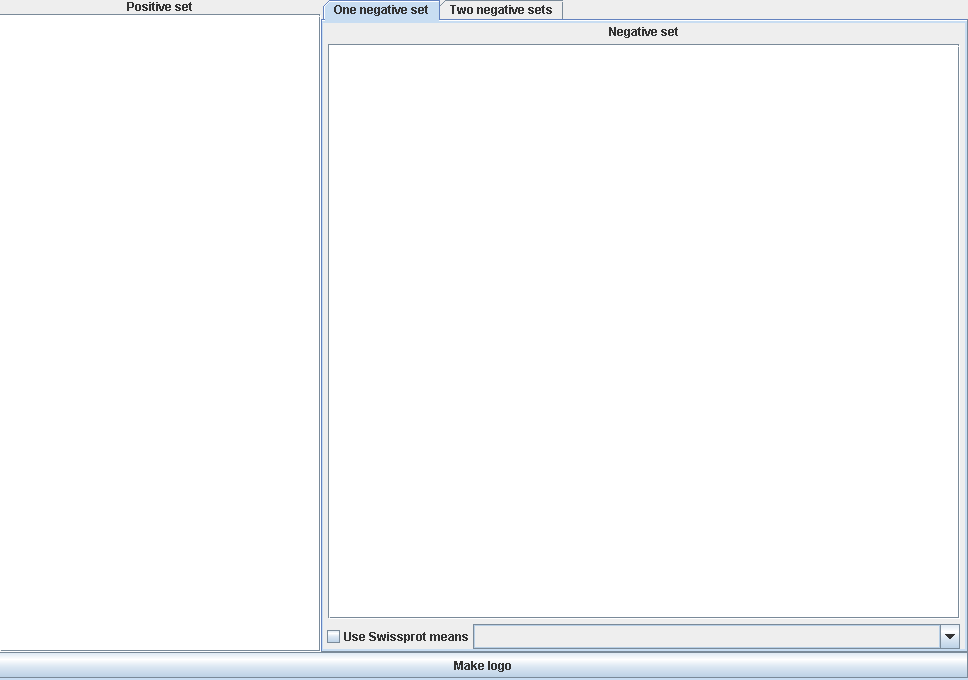
\includegraphics[scale=0.4]{static_panel.png}
\caption{The static input panel.}
\label{static panel}
\end{center}
\end{figure}

\subsection{Positive set}
\paragraph{}The positive set is in the static method always a multiple sequence alignment. The region of interest must always be located on the same position in every line and the different sequences in the multiple sequence alignment must always be of the same lenght. Gaps in the alignment will be replaced by X's. This set can be entered in the left text field on the input panel (see figure \ref{static panel})
\subsection{Reference set}
\paragraph{}Two different ways can be choosen to create a static reference set and are explained in section \ref{fixed} and section \ref{proteomal background}. Also, not one but two reference sets can be used. Two reference sets can be usefull if only at certain positions a certain technical bias is applicable. One for the first positions and one for the last positions in the positive set. The use of two negative sets can be initiated by clicking the \textit{two negative sets} tab at the right side of the frame. Then, a slider and two panels where the negative set can be defined, will be visualised. With the slider, the position where the second reference set starts and the position where the positive set will be split can be defined (see figure \ref{2negSet}).

\begin{figure}[H]
\begin{center}
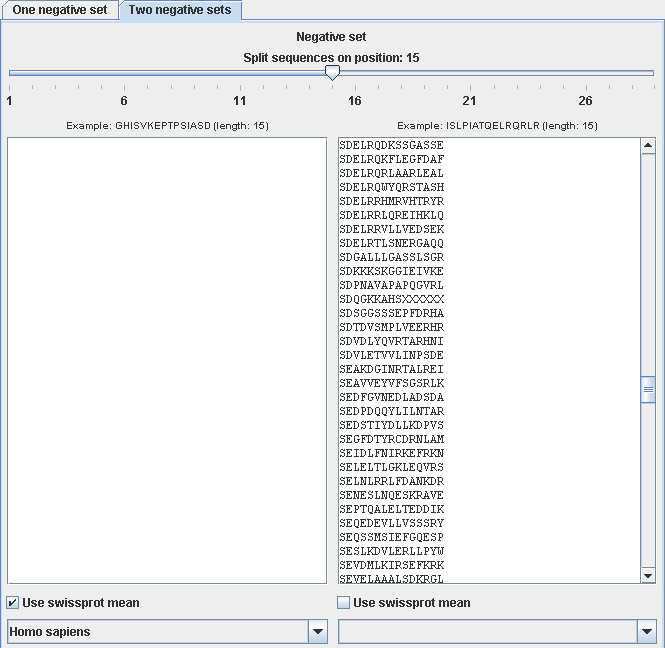
\includegraphics[scale=0.8]{2negSet.png}
\caption{The panel where a double negative set can be created. The first 15 amino acids of the positive set will be compared with the \textit{Homo sapiens} Swiss-Prot natural occurence. The last 15 amino acids of the positive set will be compared with the reference set given in the right text field.}
\label{2negSet}
\end{center}
\end{figure}

\subsubsection{Fixed reference set} \label{fixed}
\paragraph{}A user can give a multiple sequence alignment as a reference set. This negative set can be set in the large text field in the \textit{negative set} tab.
\subsubsection{Proteome background reference set} \label{proteomal background}
\paragraph{}Predifined negative sets are stored in iceLogo. For every species in the Swiss-Prot protein database the proteins will be collected and the frequency of every amino acid will be calculated. Adding a species can be done with the species adder (see section \ref{species adder}). The proteome background can be used by clicking the \textit{use Swiss-Prot mean} checkbox and by defining the species to use in the drop-down box next to or below the checkbox.
\subsection{Statistics used} \label{fixedStats}
\paragraph{}Different parameters must be calculated before iceLogo can decide if hte presence of a specific amino acid at a specific position is significant.
\begin{description}
\item[Sample size] The sample size is of great importance in the calculation of the standard deviation. The sample size is defined by the positive set and the reference set. When the sets are both multiple sequence alignments, the smallest set size (the multiple sequence alignment with the least sequence lines) will be used as the sample size. If the reference set is created with the proteome background method, the size of the positive set will be used as the sample size.
\item[Standard deviation] The standard deviation ($\sigma$) uses the sample size (N) and the frequency (f\%) of an amino acid in the the reference set and is calculated with formula \ref{sd}.
\end{description}

\begin{equation}
\sigma = \sqrt{\dfrac{f\%}{N}}
\label{sd} 
\end{equation}
\paragraph{}This calculated standard deviation will be used to calculate significances in the different visualization methods.

\section{Sampling} \label{sampling}
\paragraph{}The second method, creating the reference set from a FASTA file, can be chosen by clicking on 
\includegraphics[scale=0.4]{sampling_icon.png}. Applying the sampling method requires more parameters then the static method. As such, icelogo guides the user through these steps in a convenient 3-step wizard.

\begin{description}
\item[Step 1] assists the creation of the reference set and the user is therefore required to define which sampling strategy should be used and which FASTA file reflects the protein sequence background.
\item[Step 2] assists the creation of the experimental set(s) with an optional anchor position to align the sequence onto the FASTA file.
\item[Step 3] oveviews the configuration by simulating the upcoming analysis.
\end{description}

\subsection{Wizard Step 1 - The Reference set}

\begin{figure}[H]
\begin{center}
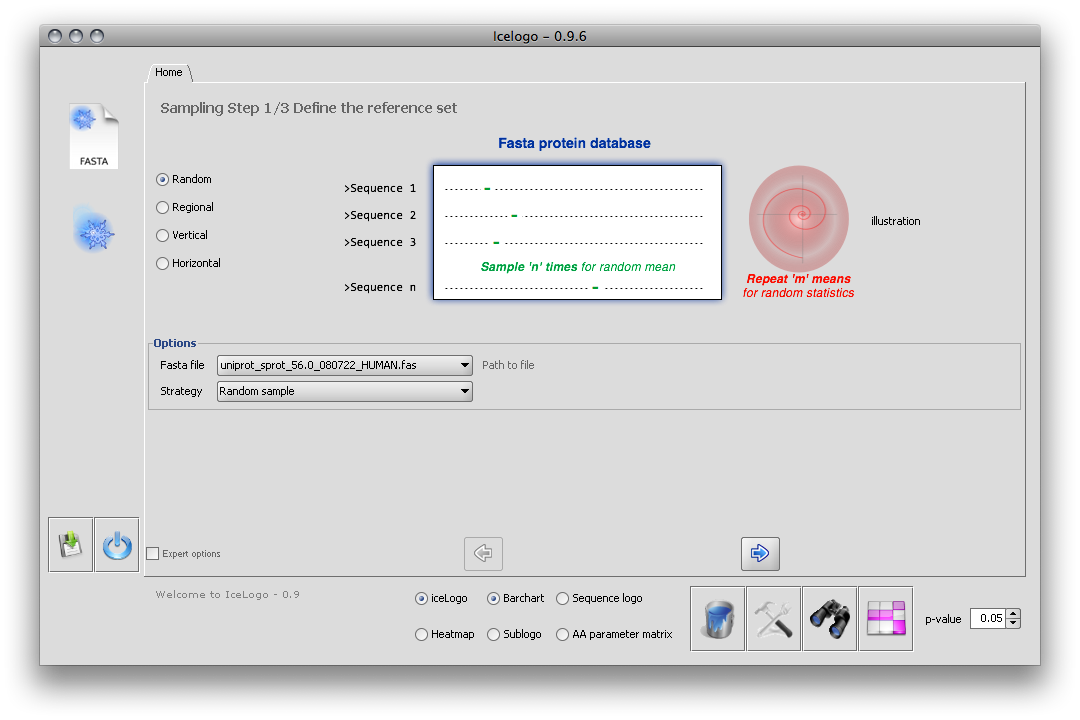
\includegraphics[width=\textwidth]{sampling_reference.png}
\caption{This figure illustrates the first wizard step of the sampling analysis in iceLogo}
\label{wizard_reference1}
\end{center}
\end{figure}

\paragraph{}	Sampling from a FASTA file comes both with advantages and drawbacks. When using static amino acid frequencies, one assumes that amino acid usage is generally equal to that of the whole proteome. But since this assumption is not actively tested by static methods, these methods might be prone to error.
Therefore the major advantage of sampling from a FASTA sequence database is such that (unexpected) variation in amino acid usage is included in the sampling test. For example, Crooks et al. published in 2004 on deviating amino acid usages  at protein extremities. Or else, amino acids have an elevated probability to repeat themselves, which might  lead an increased translation efficiency. Both examples could lead to unwanted statistical interaction and invalid conclusions. 
\paragraph{}	The major drawback is that the FASTA file must be repeatedly accessed and this computation comes with a time cost. Compared to instantaneously creating a static reference set, the sampling from the human subset of Swiss-Prot might last a minute or more.
\paragraph{}	Since we reckoned that the retrieval of a FASTA sequence database might be difficult for a layperson, icelogo also comes with an easy-to-use FASTA retrieval application. 

\subsubsection{Statistics}
The reference set is the backbone for the statistics by reflecting the probability of finding an amino acid (AA) at random or under certain conditions. This is done as following. If the experimental set contains $n$ peptides, iceLogo samples $n$ peptides from a FASTA file and thereby calculates individual amino acid frequencies. If this process is iterated for at least 30 times, then the central limit theorem tells us we are allowed to infer normally distributed reference statistics with a mean and a standard deviation for each amino acid (\ref{eq_normal_dist_aa}). Finally the experimental sequence set, also containing n peptides, can then be tested against this reference distribution and conclusions can be drawn in terms of probability (\ref{eq_prob_aa}) by performing a $t$-test.

\begin{equation}\label{eq_normal_dist_aa}
N \left( \mu_{AA},\sigma_{AA} \right)
\end{equation}

\begin{equation}\label{eq_prob_aa}
P(AA) = \frac{1}{{\sigma_{AA} \sqrt {2\pi } }}e^{{{ - \left( {x - \mu_{AA} } \right)^2 } \mathord{\left/ {\vphantom {{ - \left( {x - \mu_{AA} } \right)^2 } {2\sigma_{AA} ^2 }}} \right. \kern-\nulldelimiterspace} {2\sigma_{AA} ^2 }}}
\end{equation}
      

\subsubsection{Sampling Types}\label{sampling_statistics}
\paragraph{}	iceLogo has various algorithms to sample peptides from the FASTA file. These are the so called sampling types which the user can choose and are listed below.
\paragraph{}	Among the distinct algorithms, the following variables are common:
\begin{description}
\item[sample size $n$] equals the number of peptides to calculate a single $Freq_{AA}$ per amino acid.
\item[iteration size $i$] equals the number of times the former calculation is iterated to estimate the mean $\bar{\mu}_{AA}$ and the standard deviation $\bar{\sigma}_{AA}$  on the frequency per amino acid.  
\end{description}
 

\begin{description}
\item[]
%Explains the random sampling.
\paragraph{Random}	The random sampling method calculates the probability to encounter an amino acid at random in the FASTA file. \\To do this, the algorithm reads $n$ protein sequences at random from the FASTA file. In each protein sequence, one amino acid is chosen at random and added to an amino acid counter. When $n$ amino acids have been added to this counter the $Freq_{AA}$ per amino acid is calculated. This process is then iterated $i$ times to estimate $\bar{\mu}_{Random_{AA}}$ and standard deviation $\bar{\sigma}_{Random_{AA}}$.
\begin{figure}[H]
\begin{center}
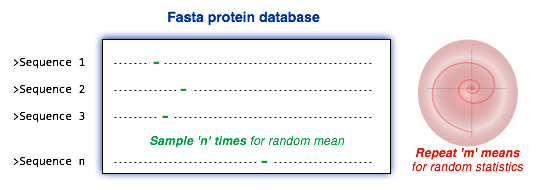
\includegraphics[scale=0.8]{random.png}
\caption{This figure illustrates the random sampling algorithm.}
\label{sampling_random}
\end{center}
\end{figure}

\item[]
\paragraph{Terminal}\label{Terminal}	The terminal sampling method calculates the probability to encounter an amino acid at a given distance from a protein terminus in the FASTA file. \\To do this, the algorithm reads $n$ protein sequences at random from the FASTA file. In each protein sequence, a terminal peptide is retrieved (N-term or C-term) with length $l$ equal to the number of amino acids in an experimental peptide. The amino acids are added to $l$ separate amino acid counter for each position. When $n$ terminal peptides and their amino acids have been added to these counters, the $Freq_{AA_l}$ per amino acid is calculated for each position. This process is then iterated $i$ times to estimate $\bar{\mu}_{Terminal_{AA_l}}$ and standard deviation $\bar{\sigma}_{Terminal_{AA_l}}$.
%Explains the terminal sampling.
\begin{figure}[H]
\begin{center}
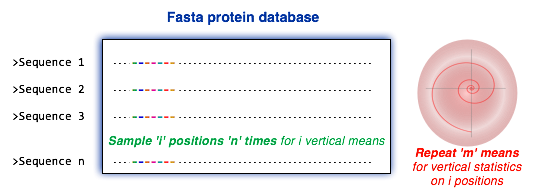
\includegraphics[scale=0.8]{terminal.png}
\caption{This figure illustrates the terminal sampling.}
\label{sampling_terminal}
\end{center}
\end{figure}

\item[]
%Explains the regional sampling.
\paragraph{Regional}	The regional sampling method calculates the probability to encounter an amino acid in the region around an anchored experimental position. \\To do this, the algorithm first analyses the amino acid frequency at an anchored position $Freq_{AA_anchor}$  in the experimental set. For example, a experimental sequence set with phosphorylated peptides anchored to the phosphorylation site has $Freq_{AA_{Ser}} =70\%$ and $Freq_{AA_{Thr}} =30\%$. Then the algorithm reads $n$ protein sequences at random from the FASTA file. In each protein sequence, a regional peptide around the anchor site is retrieved with length $l$ equal to the number of amino acids in an experimental peptide. In the example, $0.70\:x\:n$ regional peptides have a Ser anchor and $0.30\:x\:n$ regional peptides have a Thr anchor. The amino acids are then added to $l$ separate amino acid counter for each position around the anchor site. When $n$ regional peptides and their amino acids have been added to these counters, the $Freq_{AA_l}$ per amino acid is calculated for each position around the anchor. This process is then iterated $i$ times to estimate $\bar{\mu}_{Regional_{AA_l}}$ and standard deviation $\bar{\sigma}_{Regional_{AA_l}}$.
\begin{figure}[H]
\begin{center}
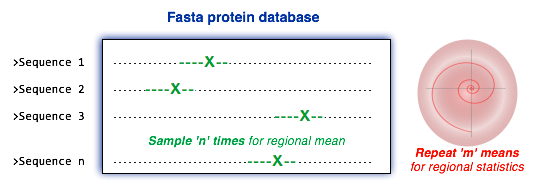
\includegraphics[scale=0.8]{regional.png}
\caption{This figure illustrates the regional sampling}
\label{sampling_regional}
\end{center}
\end{figure}

\end{description}

\paragraph{}Note that other Sampling Types can be implemented due to the pluggable software architecture. If required, please post a request in the google user group (\url{http://groups.google.com/group/iceLogo}).  

\subsubsection{User input}
\paragraph{}	Understanding the different sampling types, the creation of a reference set is done by a convenient user interface as shown in \ref{wizard_reference1}.
\begin{description}
	\item[Sample type] On the left side, the sampling type is chosen by clicking the appropriate radio button.
	\item[Illustration] On the right side, the chosen sampling type is illustrated for user convenience.
	\item[Options] On the bottom side, general input options as well as sampling type options are shown.
	\begin{description}
		\item[Fasta database] The pull-down menu lists the three last used FASTA files. Select the FASTA file that should be used for the sampling analysis. If no FASTA files are listed, you must add or download a new FASTA file. To \textit{add a new FASTA file}, click the corresponding item and navigate to the file on your computer. To \textit{download a new FASTA file} click the corresponding item and wait for the FASTA downloader dialog to open (\ref{fasta_downloader}). Therein, search the appropriate species and click the \textit{Save} button to start downloading the FASTA file. iceLogo will then download the latest Swiss-Prot release and filter the species-specific proteins into a new FASTA file. This file is then stored in the \textit{../conf/} folder in the iceLogo installation path and is automatically added into the pull-down menu.
		 
			\begin{figure}[H]
			\begin{center}
			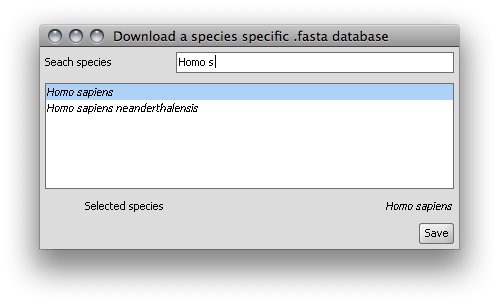
\includegraphics[width=0.5\textwidth]{fasta_download.png}
			\caption{This figure shows the FASTA downloader. Start typing a species name (ex: Homo sapiens) in the upper text field and all the matching species names will be matched. By clicking the \textit{Save} button in the bottom-right corner, the appropriate FASTA file will be retrieved from Uniprot.} 
			\label{fasta_downloader}
			\end{center}
			\end{figure}

	\end{description}
	
	\item[Expert Options] These options enable extra fine-tuning of the sampling algorithm but require more understanding of the corresponding algorithm.
	\begin{description}
		\item[Iteration size] Set the number of iterations for calculating the mean $\bar{\mu}_{AA}$ and the standard deviation $\bar{\sigma}_{AA}$  on the frequency per amino acid.
		\item[Terminal - Anchor start position] Set the offset to start terminal sampling 
		\item[Terminal - Direction] Set the direction to either sample peptides from the N- or C-terminal end of the protein. 
	\end{description}
\end{description}

\paragraph{}	If all parameters have been filled in correctly, click the next button to proceed to the second step which allows you to define the experimental set.

\subsection{Wizard Step 2 - The Experimental set}
\paragraph{}	Opposite to the first step, the second step doesn't require a lot of input: an aligned sequence set that will be tested against the reference set created by sampling a FASTA database. This aligned sequence set is typically the result of an experiment (proteolytic cleavage sites, phosphorylation, etc..) and it is therefore called the experimental sequence set.     

\subsubsection{User input}

\paragraph{One experimental set} A single experimental (aligned) sequence set can be inserted in the main textfield.

\begin{figure}[H]
  \centering
  \subfloat[Insert 1 experimenal set for \textit{Random} or \textit{Terminal} sampling]{\label{fig:exp_1_a}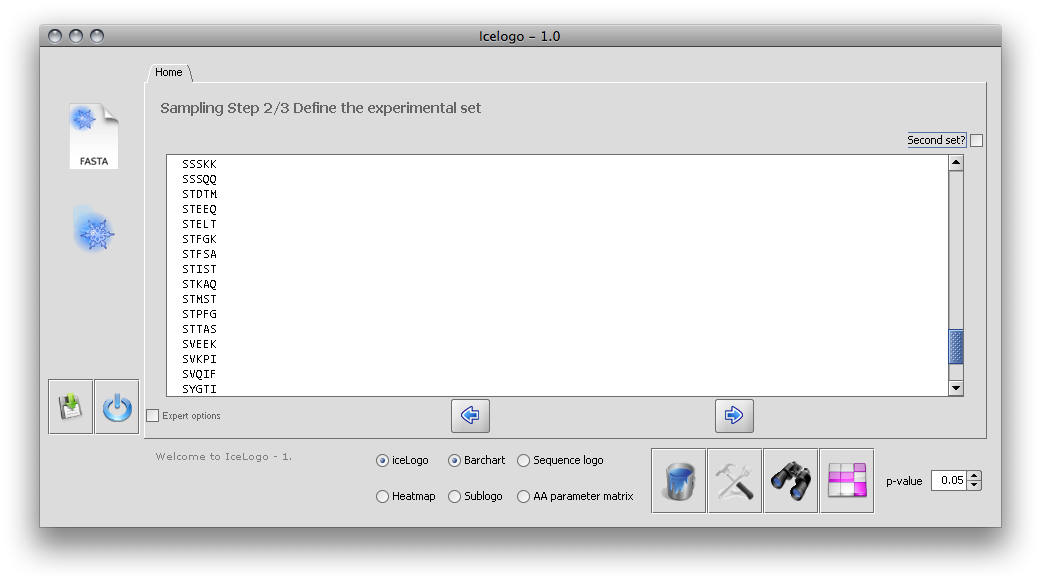
\includegraphics[width=0.8\textwidth]{exp_1.png}} \\               
  \subfloat[Insert 1 experimenal set and its anchor site for \textit{Regional} sampling]{\label{fig:exp_1_b}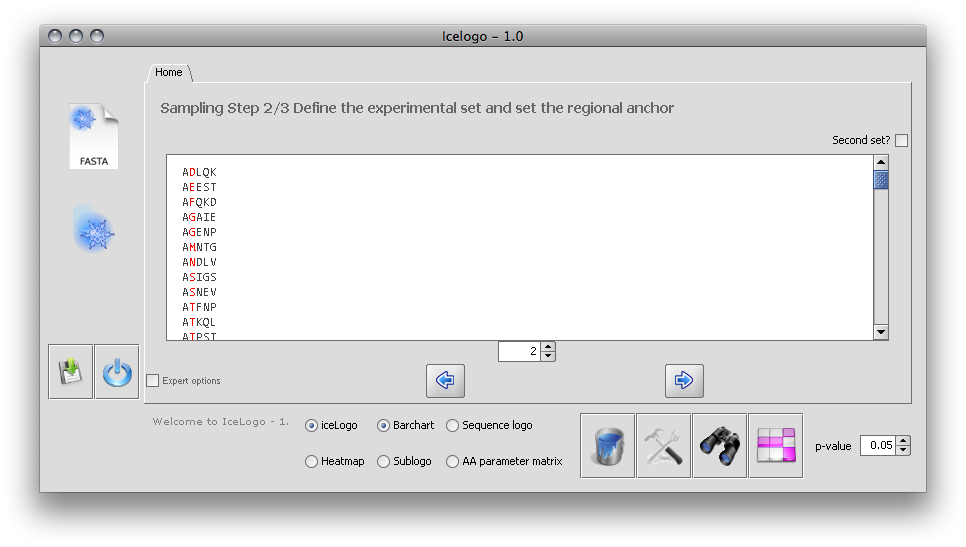
\includegraphics[width=0.8\textwidth]{exp_1_anchor.png}}
  \caption{This figure illustrates the single experimental sequence input dialog. Note that the \textit{Regional} sampling \ref{sampling_regional} also requires the user to define the anchor position.}
  \label{fig:exp_1}
\end{figure}

\paragraph{Two experimental sets}	By clicking the \textit{second experimental set} checkbox in the upper-right corner, a second experimental sequence set can be inserted. Note that not all visualizations are currently support displaying two experimental sets.

\begin{figure}[H]
  \centering
  \subfloat[Insert 2 experimenal sets for \textit{Random} or \textit{Terminal} sampling]{\label{fig:exp_2_a}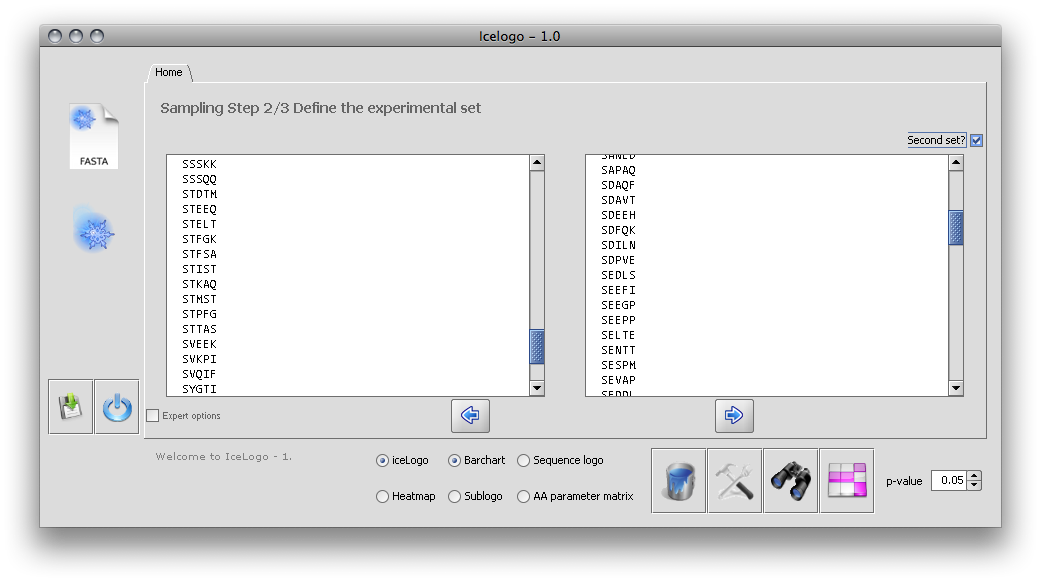
\includegraphics[width=0.8\textwidth]{exp_2.png}} \\               
  \subfloat[Insert 2 experimenal sets and its anchor site for \textit{Regional} sampling]{\label{fig:exp_2_b}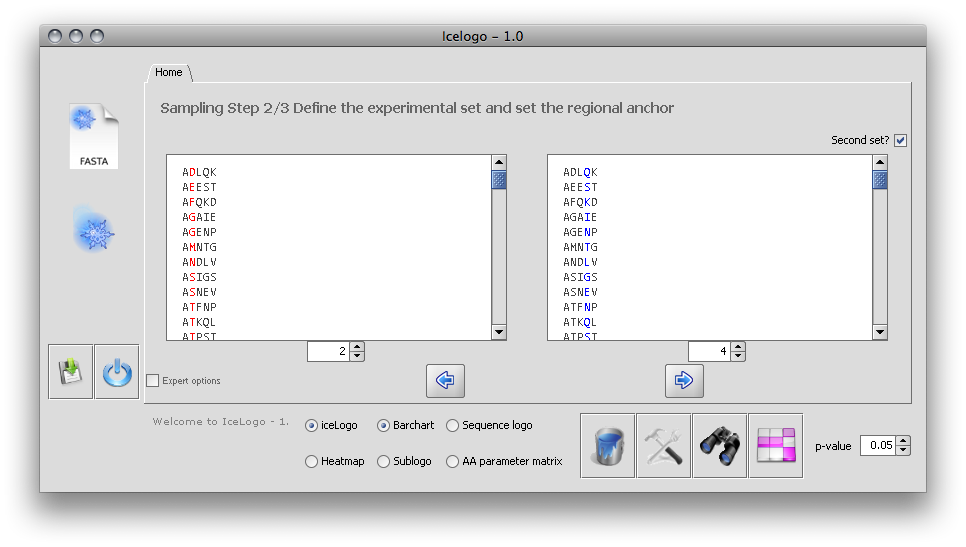
\includegraphics[width=0.8\textwidth]{exp_2_anchor.png}}
  \caption{This figure illustrates the double experimental sequence input dialog. Note that the \textit{Regional} sampling (\ref{sampling_regional}) also requires the user to define the anchor position on both sequence sets.}
  \label{fig:exp_2}
\end{figure}

\paragraph{}	If all parameters have been filled in correctly, click the next button to proceed to the third and last step which presents an overview of the upcoming analysis.

\subsection{Wizard Step 3 - The Overview}
\paragraph{}	In opposite to the former step, the Overview step requires no further input but presents - for user convenience - an aggregation of the user input gathered by the former steps.
		

\begin{figure}[H]
  \centering
  \subfloat[The overview of the reference and experimental set.]{\label{fig:overview_a} 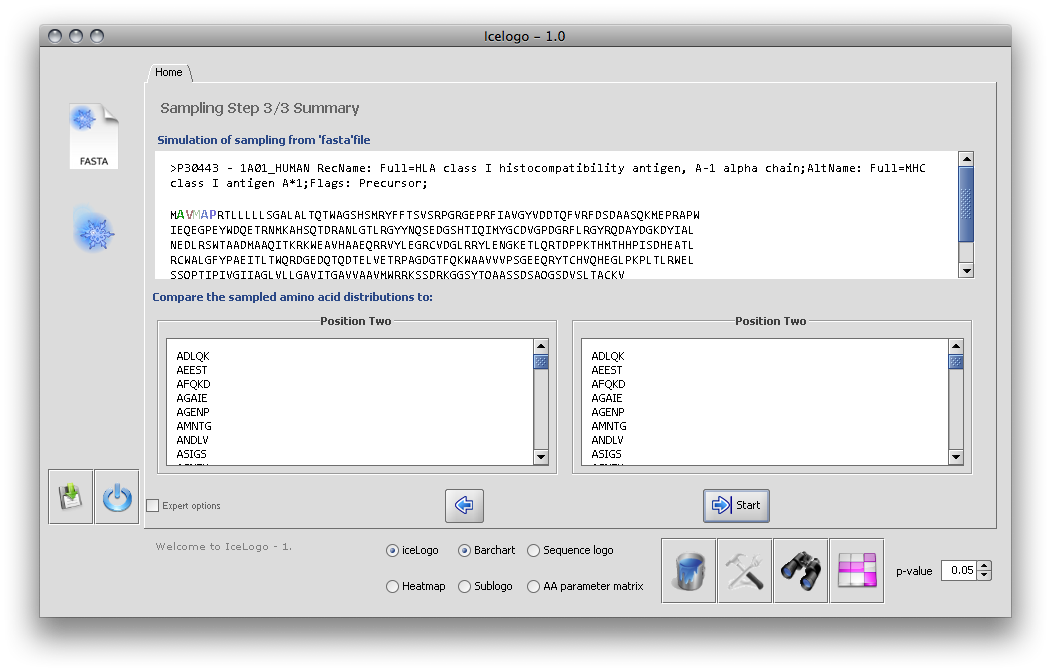
\includegraphics[width=0.8\textwidth]{overview.png}} \\               
  \subfloat[The overview of the reference and experimental set in expert mode.]{\label{overview_b}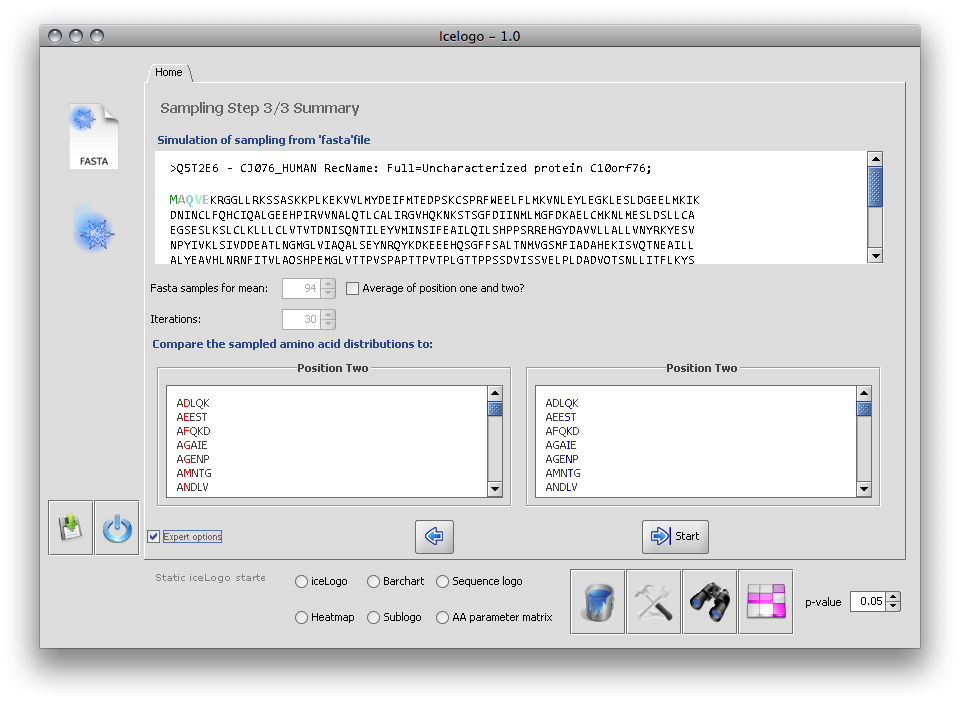
\includegraphics[width=0.8\textwidth]{overview_expert.png}}
  \caption{This figure shows the final Overview step of the sampling Wizard. The upper panel simulates protein entry reading from the FASTA file and meanwhile, color annotates the to be sampled amino acids. Every second, a new protein is displayed to illustrate the sampling process to the user. The bottom panel then shows the experimental sequence sets. In the expert mode, the middle panel also shows sample size $n$ and iteration size $i$ (\ref{sampling_statistics}). Hence both are non-editable since these values are inferred from  former input. }
  \label{fig:overview}
\end{figure}

\paragraph{Start!}	If the user agrees with the Overview, then the sampling analysis can be started by clicking the next button. Note that this can be, from a computational viewpoint, rather intensive and one should expect the sampling analysis to take one, up to a few minutes.	


%chapter on the data visualization
\chapter{Visualization methods in iceLogo} \label{output}
\paragraph{}The iceLogo program will create a framework (see chapter \ref{running}) with a positive and reference set independently of the chosen mode (static or dynamic). By this, iceLogo can use the foundation to create the different visualization methods described below.

% ICELOGO
%%%%%%%
\section{iceLogo} \label{iceLogo}
\paragraph{}An iceLogo attemps to visualize a consensus sequence in a comprehensive manner just like sequence logos. However, it has two major benefits when compared to sequence logos. First, an iceLogo will always use a reference set. When no multiple sequence alignment can be given to create a reference set the option is to use the proteome background or sample a reference set from a protein FASTA file. In this way, iceLogo always uses statistics to find over- and under-presented amino acids. Especially, the visualization of significantly under-represented amino acids is new and is not present in sequence logos. Second, the dynamic nature of iceLogos, mainly the changing of the scoring system (see below), lets the user find changes in low abundant amino acids.
\paragraph{}On the iceLogo panel, significantly under- and over-represented amino acids will be visualized. For every position, the amino acid frequencies in the positive set will be compared with the frequencies in the reference set. An amino acid will be regulated if the Z-score is not a part of the confidence interval (for the calculation of the confidence interval see \ref{p-value}). The Z-score is calculated with the formula: Z-score = $\dfrac{X - \mu}{\sigma}$. The formula will calculate how many times the frequency (X) is deviated from the mean ($\mu$, the frequency of a specific amino acid on a specific position in the reference set) in terms of the standard deviation ($\sigma$). The way these standard deviations are calculated depends on the iceLogo mode used (see chapter \ref{running}).
\paragraph{}The color of the amino acids can dynamicly be changed in the color panel (see \ref{color panel}). The amino acids will be colored pink if the amino acid is significantly regulated, and if this specific amino acid does not occure in the positive or reference set. Three different scoring systems were developed (see \ref{general parameters}) and can be dynamically changed to generate different iceLogos. If the scoring method is set to \textit{fold change}, the calculated height of a pink amino acid is infinite. Therefore, the height will be set to a specific value. Different scenarios exist for calculating this height.
\begin{itemize}
\item[] If only \textbf{one} amino acid is regulated and the calculated amino acid size is \textbf{infinite}, the height of the amino acid will be the same as the maximal height that can be visualized in the iceLogo.
\item[] If \textbf{more} amino acids are regulated and \textbf{all} the calculated amino acid sizes are \textbf{infinite}, the height of the amino acids will be the same as the maximal height that can be visualized in the iceLogo divided by the nummer of regultated amino acids on that position. All the regulated and infinite amino acids must be either over- or under-represented.
\item[] If \textbf{more} amino acids are regulated but \textbf{not all} the calculated amino acid sizes are \textbf{infinite}, the height of the infinite amino acids will 10 \% larger than the largest not infinite amino acid.
\end{itemize}
\paragraph{}The user can zoom in and out on the iceLogo by clicking the left and right mouse button respectively. The height of the Y-axis can also be manually changed in the general parameters panel (see \ref{general parameters}).
%BAR CHART
%%%%%%%%
\section{Bar Chart}
\paragraph{}	The bar chart displays absolute frequencies for all amino acids. It is inherent to the iceLogo bar chart to display a single position, therefore the user can control the position by moving the slider at the bottom of the bar chart. The black bars show the mean as calculated from the reference set, along with blue error bars showing the probability  boundaries (defined by the p-value in the bottom right corner).
\paragraph{}	As such, the user is forced to reflect on large standard deviations when using small experimental data sets. Also, if the experimental data set grows, the error bars shrink. Taken together, absolute means for every amino acids and their error are best viewed in the bar chart.

\begin{figure}[H]
	\begin{center}
	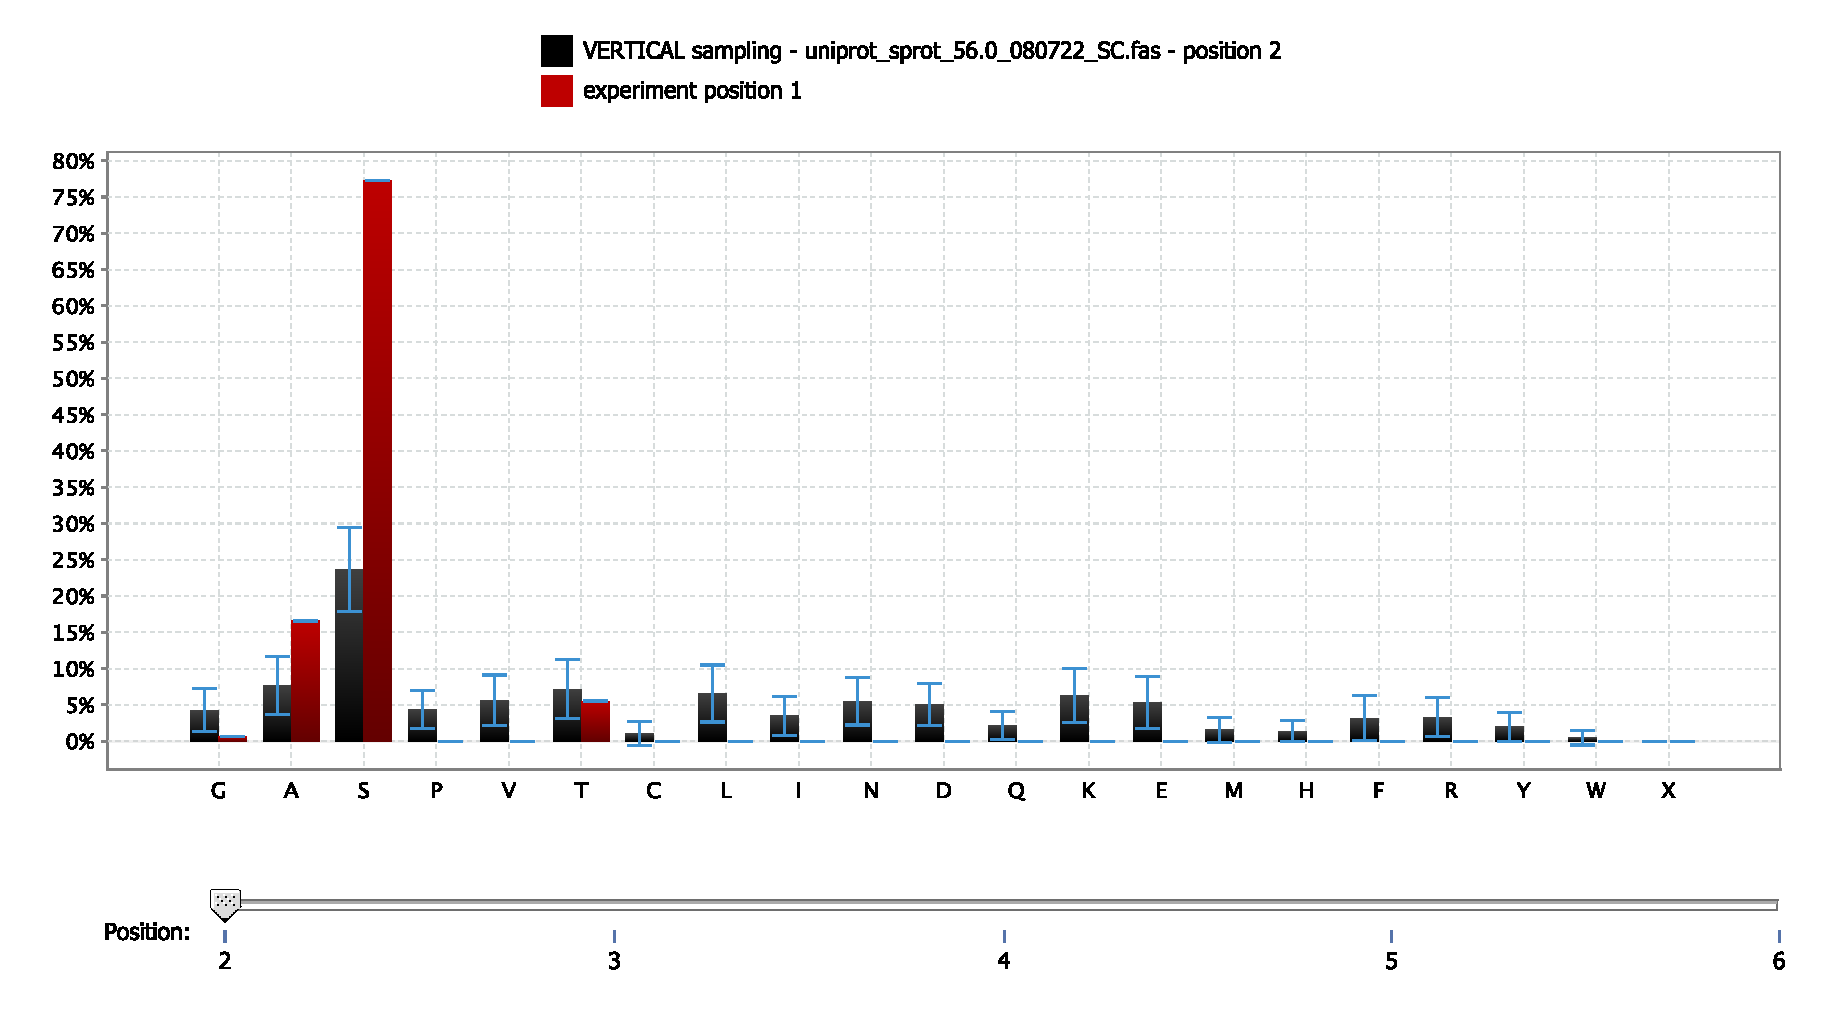
\includegraphics[width=0.8\textwidth]{barchart.pdf}
	\caption{The figure shows the bar chart visualisation of an iceLogo analysis. The bar chart is a position specific image and the index of the position can be moved by the slider in the bottom. The top of the bar chart shows a legend of the bars. The black bar represents the amino acid frequency mean and standard deviation within the reference set. The black bars are aligned with colored bars indicating the amino acid frequency within the experimental set.}
	\label{fig:barchart}
	\end{center}
\end{figure}


%HEAT MAP
%%%%%%%
\section{Heat map}
\paragraph{}A heat map attempts to visualize all the amino acid occurrences for all positions in one picture. The heat map is a 2D data matrix where every row is an amino acid and every column a position. At the right side of the heat map the gradient shows which p-values correlates with which colour. The Z-score is used for the calculation of the position and amino acid specific p-value and is calculated with the formula: Z-score = $\dfrac{X - \mu}{\sigma}$. The formula will calculate how many times the frequency (X) of that amino acid on that position is deviated from the mean ($\mu$, the frequency of a specific amino acid on a specific position in the reference set) in terms of the calculated standard deviation ($\sigma$). An error function (see formula \ref{erf}) can calculate a p-value for this Z-score.

\begin{equation}\label{erf}
P-value = erf(\dfrac{Z-score}{\sqrt{2}})
\end{equation}

\paragraph{}One cell in the heat map matrix will be coloured according to the calculated p-value for that position and amino acid. Only significantly up- and down-regulated elements - according to the given p-value (see \ref{p-value} for setting this p-value) - are coloured in respectively a shade of green and red. The non-regulated elements are coloured black.


\begin{figure}[H]
	\begin{center}
	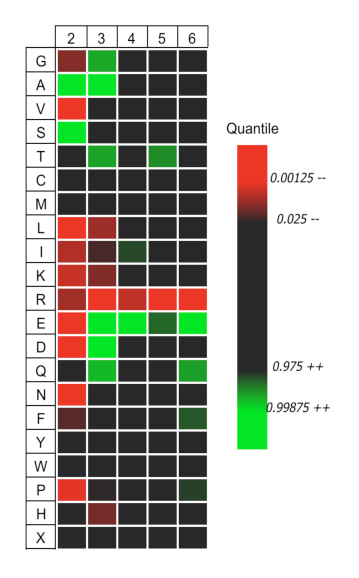
\includegraphics{heatmap.pdf}
	\caption{The figure shows the heatmap result of an iceLogo analysis. Increased or decreased amino acid frequencies are shown in a gradient of respectively green or red shades.}
	\label{fig:heatmap}
	\end{center}
\end{figure}

\paragraph{}If the heat map is larger than the displayed screen, it can be visualized by first clicking on the heat map and secondly navigating with the arrow keys.

%SEQUENCE LOGO
%%%%%%%%%%%
\section{Sequence logo} \label{sequence logo}
\paragraph{}Sequence logos were originally created by Schneider and Stephens in 1990 and are used to visualize consensus sequences. Sequence logos are based on the \textit{information theory}. This theory states that a \textit{bit} is the amount of information necessary to choose between two equally probable choices. In a sequence logo the height of a stack of amino acids is thus calculated and presented in \textit{bits}. The height of one amino acid in such a stack reflects its frequency. 
\paragraph{}The maximal height of the stack is calculate with formula \ref{maxbits}. Where \textit{choices} stands for the number of possibile items. For DNA and RNA this is 4 and thus resulting in a maxBits value of 2. For proteins, there are 20 choices (amino acids) and the resulting maxBits is 4.32.
\begin{equation}
maxBits = \log_{2} choices
\label{maxbits} 
\end{equation}
\paragraph{}The final sequence logo height (sH) is calculated with formula \ref{sH}. In formula \ref{sH} the maxBits is substracted with the calBits. This calBits is calculated with formula \ref{calBits}. P$_{i}$  stands for the frequency of amino acid \textit{i}.
\begin{equation}
maxBits - calBits =sH
\label{sH} 
\end{equation}

\begin{equation}
calBits = - \Sigma (P_{i} \log_{2} P_{i})
\label{calBits} 
\end{equation}
\paragraph{}As a simple example, a set of 50 Arg (R) and 50 Lys (K) were used to create a sequence logo. The frequency of these amino acids are in both cases 50\%. Formula \ref{calBits} is used to calculate the calBits resulting in  1 (see formula \ref{calBitsTryp}).
\begin{equation}
calBits = 1 = - [ 0.5 \log_{2}(0.5) + 0.5 \log_{2}(0.5)]
\label{calBitsTryp} 
\end{equation}
The final sequence logo height can be calculated using formula \ref{sH}; 4.32 - 1 = 3.32. The height of the sequence logo in figure \ref{slTryp}.A is indeed 3.32.
\paragraph{}The iceLogo program can use the reference set for a background correction in sequence logos. iceLogo will calculate the height of the stack in the reference set and will substract it of the height of the stack in the positive set. This corrected sequence logo is presented in figure \ref{slTryp}.B.

\begin{figure}[H]
\begin{center}
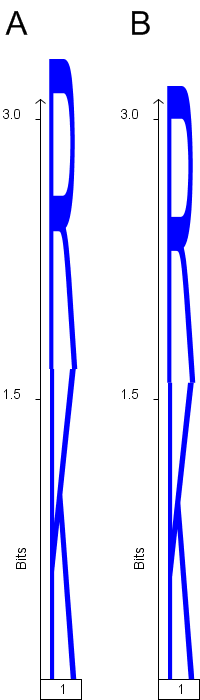
\includegraphics[scale=0.3]{slTryp.png}
\caption{These are both sequence logos generated with the iceLogo tool. Figure A is the normal sequence logo. Figure B is the reference set corrected sequence logo. Here the reference set is the human Swiss-Prot proteome.}
\label{slTryp}
\end{center}
\end{figure}

\paragraph{}10000 random human peptides were generated for the following example. The sequence logo without correction is given in figure \ref{10000random}.A. Figure \ref{10000random}.B gives the sequence logo with reference set correction. With this example, it's clearly shown that a background reduction in sequence logos has an important effect.

\begin{figure}[H]
\begin{center}
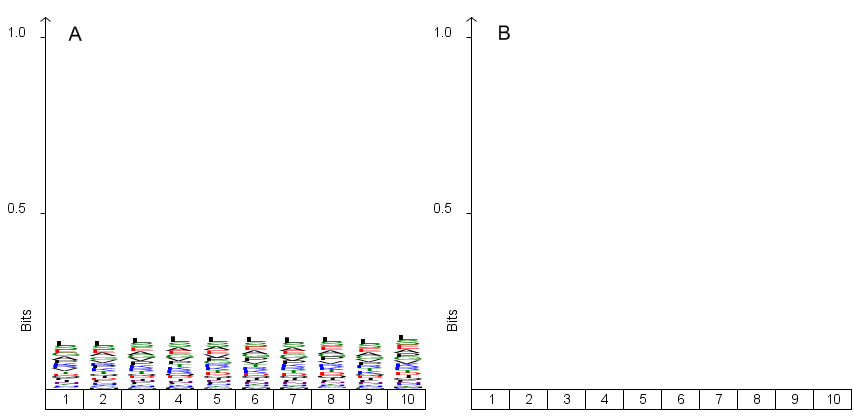
\includegraphics[scale=0.4]{10000random.png}
\caption{These are both sequence logos generated with the iceLogo tool. Figure A is the normal sequence logo. Figure B is the reference set corrected sequence logo. Both were created with 10000 random human peptides.}
\label{10000random}
\end{center}
\end{figure}

\paragraph{}The user can again zoom in and out by clicking the left and right mouse button.  A sequence logo cannot be generated when two experimental sets are compared in the sampling method.


%SUB LOGO
%%%%%%%%%%%
\section{subLogo}
\paragraph{}In the subLogo tab, the user can try to find hidden elements in the data. The subLogo frame is presented in figure \ref{subLogo}. In this frame a smaller version of the iceLogo program is run. The user can select a positive set, which is a part of the total positive set. Two ways exist of creating this positive set.
\begin{itemize}
\item[1.] The user can select one of the positively regulated amino acids listed in the upper left part of the subLogo tab.
\item[2.] The user can select a specific (both regulated and non-regulated) amino acid with the drop-down box and can select a specific position with the position slider both at the left site of the tab.
\end{itemize}
In both cases, the positive set will be a subselection of the totale positive set where at a specific position, a specific amino acid is present.
\paragraph{}The negative set can be created using the totale experimental set or by choosing a Swiss-Prot composition. By default an iceLogo and a bar chart are created. Also, a panel with the subselection of the positive set is created.
\paragraph{}The different created panels can be saved by using the \textit{save subLogo} button. 

\begin{figure}[H]
\begin{center}
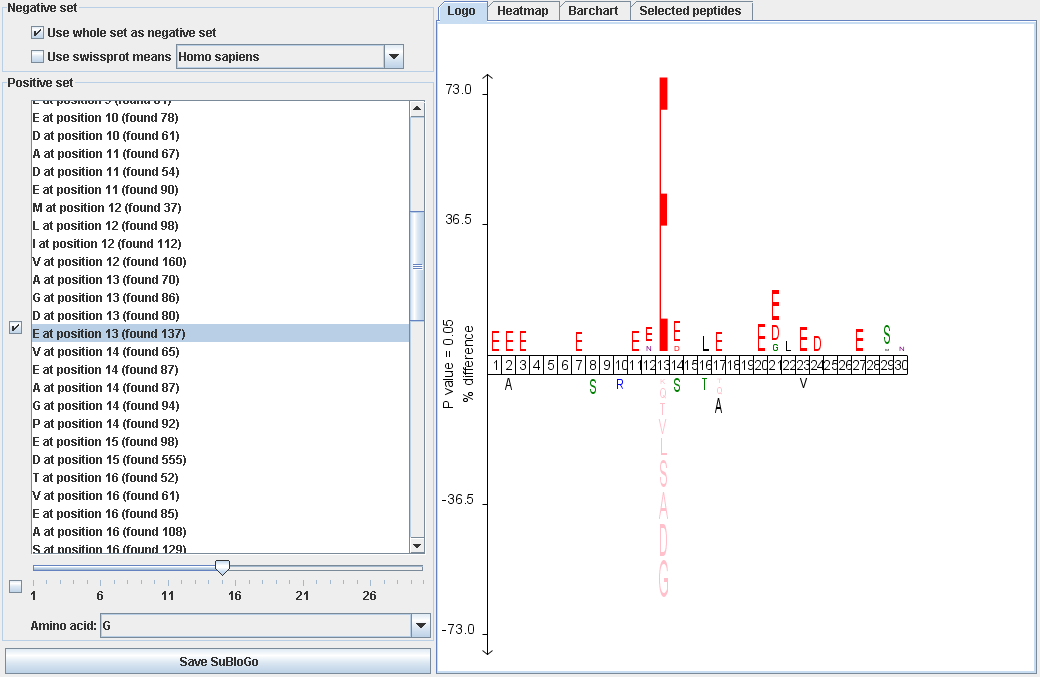
\includegraphics[scale=0.7]{subLogo.png}
\caption{The subLogo tab.}
\label{subLogo}
\end{center}
\end{figure}



% AA PARAMETER
%%%%%%%%%%
\section{Amino acid parameter graph}
\paragraph{} The iceLogo program can visualize amino acid parameters. These parameters can be found in the AAindex1 database (\url{http://www.genome.jp/aaindex/}). The AAindex database is a database of numerical indices representing various published physicochemical and biochemical properties of amino acids. Currently, 544 indices are stored as matrices in this database and can be visualised by iceLogo. One of these 544 indices can be choosen in the Aa parameter chooser (see \ref{Aa parameter chooser}).
\paragraph{}The value for a specific position is calculated with formula \ref{aa} where P$_{i}$ is the frequency for amino acid \textit{i} and V$_{i}$ is the value for amino acid \textit{i} in the  amino acid parameter matrix used for the creation of the amino acid parameter graph. The values for different positions from the experimental set are linked by a green line. If two experimental sets are being analyzed, then this second set is linked by a blue line.
\begin{equation}
\Sigma P_{i} * V_{i}
\label{aa} 
\end{equation}
\paragraph{}A sliding window can be used to smoothen the green line that connects the values for the different positions. The minimal size of the sliding window is 2. The sliding window size can be set in the amino acid parameter chooser panel (see \ref{Aa parameter chooser}). The value on each position is the mean of the different positions used. In the following table, the positions used for a specific position in the graph are listed for the window sizes 3 and 4.

\begin{center}
\begin{tabular}{ccccccccccc}
 &  &  \multicolumn{8}{c}{Position in graph } \\ 
\cline{3-10} 
 &  & 1 & 2 & 3 & 4 & \ldots & 28 & 29 & 30 \\ 
 &  &  \multicolumn{8}{c}{Positions used} \\ 
\cline{3-10} 
\raisebox{-1ex}{window} & 3 & \textbf{1} & 1,\textbf{2} & 1,2,\textbf{3} & 2,3,\textbf{4} & \ldots & 26,27,\textbf{28} & 27,28,\textbf{29} & 28,29,\textbf{30} \\ 
\raisebox{1ex}{size} & 4 & \textbf{1},2 & 1,\textbf{2},3 & 1,2,\textbf{3},4 & 2,3,\textbf{4},5 & \ldots & 26,27,\textbf{28},29 & 27,28,\textbf{29},30 & 28,29,\textbf{30} \\
\end{tabular} 
\end{center}

\paragraph{}The reference set is used to create a pink zone on the graph. This zone represents the non-regulated region. This non-regulated zone (the confidence interval) is determinded by the p-value (see \ref{p-value}) and the background standard deviation. Two ways exist to create this background standard deviation.
\begin{enumerate}
\item When the static iceLogo method is used (see \ref{static}) a standard deviation will be calculated for every position. This standard deviation will be calculated on 100 means. One such a mean, is the mean of the amino acid parameter values for N random (based on the reference set) amino acids and N is the sample size (see \ref{fixedStats} for the sample size calculation). This way, the reference set is used to simulate the background for an amino acid parameter.
\item When the sampling iceLogo method is used (see \ref{sampling}), a background standard deviation will be calculated for every position. This standard deviation will be calculated on X parameter value means. X is the dimension of sampling. One such a mean, is the mean of the sampled amino acids parameter for a specific dimension. This way, the reference set is used as the background for an amino acid parameter. 
\end{enumerate} 
The red line in the pink zone represents the mean of the means used for the calculation of the background standard deviation.

% CORRELATION LINE
%%%%%%%%%%
\section{Correlation line}
\paragraph{} The iceLogo program can visualize the correlation between the different amino acids on one position. The correlation is calculated by using a substitution matrix. These substitution matrices can be found in the AAindex2 database (\url{http://www.genome.jp/aaindex/}). A substitution matrix holds values that describe the rate in which one amino acid changes in another amino acid over time. Currently, 94 substitution matrices are in this database and can be visualised by iceLogo. One of these can be choosen in the general parameter frame (see \ref{general parameters}).
\paragraph{}For every amino acid in the set, the substitution score is calculated by tacking the mean of the substitution values of this amino acids with all the other amino acids in the set on that position. A substitution score is not normalized when the substitution score for one amino acid is multiplied by the substitution value of this amino acid with itself. If the set has 100 amino acids, 99 substution scores will be calculated for every amino acid. The mean of these 99 substitution score for the different positions from the experimental set are linked by a green line. If two experimental sets are being analyzed, then this second set is linked by a blue line.

\paragraph{}The reference set is used to create a gray zone on the graph. This zone represents the non-regulated region. This non-regulated zone (the confidence interval) is determinded by the p-value (see \ref{p-value}) and the background standard deviation. Two ways exist to create this background standard deviation.
\begin{enumerate}
\item When the static iceLogo method is used (see \ref{static}) a standard deviation will be calculated for every position. This standard deviation will be calculated on 100 substitution means. One such a mean, is the mean of the amino acid substitution values for N random (based on the reference set) amino acids and N is the sample size (see \ref{fixedStats} for the sample size calculation). This way, the reference set is used to simulate the background.
\item When the sampling iceLogo method is used (see \ref{sampling}), a background standard deviation will be calculated for every position. This standard deviation will be calculated on X parameter value means. X is the dimension of sampling. One such a mean, is the mean of the sampled amino acids parameter for a specific dimension. This way, the reference set is used as the background for an amino acid substitution. 
\end{enumerate} 
The dark line in the grey zone represents the mean of the means used for the calculation of the background standard deviation.

%chapter on the parameters that can be set in iceLogo
\chapter{Parameters}
\section{Choosing visualization output}
\paragraph{} The different types of output (listed below and discussed in chapter \ref{output}) can be selected at the lower end of the frame. The iceLogo and the barchart are selected by default.
\begin{itemize}
\item[] $\boxtimes$ iceLogo
\item[] $\boxtimes$ Bar chart
\item[] $\square$ Heat map
\item[] $\square$ Sequence logo
\item[] $\square$ subLogo
\item[] $\square$ Aa parameter graph
\end{itemize}
\section{P-value} \label{p-value}
\paragraph{}The p-value is used in all the different frames and can be set by changing the spinner-box which is located at the right bottom of the screen. The default p-value is 0.05.
The confidence interval can be calculated with this p-value using the Wichura algorithm. In the following table some confidence intervals in function of the standard deviation ($\sigma$) are given for p-values.

\begin{center}
\begin{tabular}{|c|c|}
\hline p-value &  $<$ Z-score \\ 
\hline \ldots & \ldots  \\ 
\hline 0.20 & [-1.28 $\sigma$; 1.28 $\sigma$] \\ 
\hline 0.10 & [-1.65 $\sigma$; 1.65 $\sigma$] \\ 
\hline 0.05 & [-1.96 $\sigma$; 1.96 $\sigma$] \\ 
\hline 0.02 & [-2.33 $\sigma$; 2.33 $\sigma$] \\ 
\hline 0.01 & [-2.58 $\sigma$; 2.58 $\sigma$] \\ 
\hline 0.005 & [-2.81 $\sigma$; 2.81 $\sigma$] \\ 
\hline \ldots & \ldots  \\ 
\hline 
\end{tabular} 
\end{center}

\section{Amino acid color} \label{color panel}
\paragraph{}The color of the amino acids used in the iceLogo and sequence logo (see sections \ref{iceLogo} and \ref{sequence logo}) can be changed. This can be done in the panel that opens after the \textit{Amino acid color} 
\includegraphics[height=5ex]{color.png} button is pushed.

\section{General parameters} \label{general parameters}
\paragraph{}Some general parameters can be set in the panel that opens upon clicking the \textit{general iceLogo parameter} 
\includegraphics[height=5ex]{param.png} button. These different parameters will be described in the following and can be seen in figure \ref{gen_param}.
\par

\begin{figure}[H]
\begin{center}
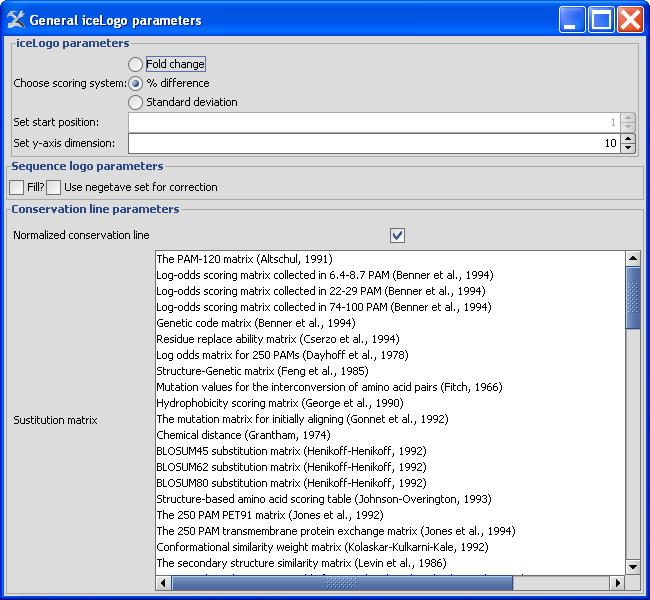
\includegraphics[scale=1.0]{gen_param.png}
\caption{The general iceLogo parameter panel.}
\label{gen_param}
\end{center}
\end{figure}

\begin{description}
\item[Choosing scoring system] Different scoring methods can be used in an iceLogo (see section \ref{iceLogo}). The scoring method has an effect on the size of a regulated amino acid and the vertical position in the stack of regulated amino acids.

\begin{itemize}
\item \textbf{Fold change} When this method is selected the fold change will determine the size of the amino acid. In the following table the frequencies of two amino acids with their fold change are given. Although the percentage difference between the positive and the reference set is for both amino acid the same (6\%), the fold changes of the two amino acid show a large difference (7 $\Longleftrightarrow$ 2). The fold change scoring method let the user thus look for the regulation of low abundance amino acids.

\begin{center}
\begin{tabular}{c|c c}
Type & AA$_{1}$ & AA$_{2}$\\ 
\hline Frequency in experimental set (F+) & 7\%  & 12\% \\
Frequency in reference set (F-) & 1\% & 6\% \\ 
Percentage difference & 6\% & 6\% \\ 
Fold change $\dfrac{F+}{F-}$ & \textbf{\textit{7}} & \textbf{\textit{2}}\\ 
\end{tabular} 
\end{center}

If the calculated fold change (FC) is smaller than 1 the fold change will be converted via formula \ref{changeFC} to the converted fold change (FC$_{con}$). By this, the height of negatively regulated amino acid can be compared with the height of positively regulated amino acids. 
\begin{equation}
FC_{con} = \dfrac{1}{FC} * -1
\label{changeFC} 
\end{equation}
The following table gives an example of a converted fold change.
\begin{center}
\begin{tabular}{c|cc}
 & AA$_{1}$ & AA$_{2}$ \\
\hline Frequency experimental set (F+) & 12\% & 6\% \\
Frequencey reference set (F-) & 6\% & 12\% \\
Fold change (FC = $\dfrac{F+}{F-}$) & 2 & 0.5 \\
Converted fold change (FC$_{con}$) & 2 & \textbf{-2} \\
\end{tabular} 
\end{center}


\item \textbf{Percentage difference} This simple scoring method used the difference in frequency for an amino acid in the experimental set and the reference set as a measure of the height of a letter in the amino acid stack. This is the default scoring method.
\item \textbf{Standard deviation} The Z-score of an amino acid is used as a measure of the size of a letter in the amino acid stack. The Z-score is calculated with the formula: Z-score = $\dfrac{X - \mu}{\sigma}$. The formula will calculate how many times the frequency (X) is away from the mean ($\mu$) in terms of standard deviation ($\sigma$). The height of the letter will be correlated to the Z-score.
\end{itemize}
\item[Start position] The start position used in the different visualization panels can be set with the spinner. The default value is 1. The start position cannot be changed manually if the iceLogo program is run in the sampling mode.
\item[Y-axis height] The height of the visible part of the Y-axis in the iceLogo (see \ref{iceLogo}) can be set manually with the spinner. Left and right clicking on the iceLogo will also change this value.
\item[Sequence logo parameters] Two parameters can be used in the creation of the sequence logo.
\begin{itemize}
\item \textbf{Fill} On the sequence logo panel a filled logo will be created if the \textit{fill} checkbox is selected. A filled logo is a stack of amino acids for every position. The height of every stack is 100\%. The height of every amino acid is related to its frequency. No statistics are used in this panel and all, and not only the significant amino acids, are visualised.
\item \textbf{Use reference set correction} When this checkbox is selected a sequence logo for the reference set will be calculated. The height of the stack (in \textit{bits}) in the experimental set will be substracted with the calculated height of the stack in the reference set. See \ref{sequence logo} for examples.
\end{itemize}
\item[Conservation line parameters] In this part of the panel the substitution matrix can be chosen. It can also be selected here that the conservation line should be normalized.


\end{description}

\section{Aa parameter chooser} \label{Aa parameter chooser}
\paragraph{}The amino acids parameter chooser opens after the \textit{chooser} 
\includegraphics[height=5ex]{aaparam.png} button is clicked. In the amino acid parameter chooser (see figure \ref{Aa_paramter_chooser}), the list of 544 indices in the AAindex1 database can be searched. This is done by typing a search term in the text field at the top of the panel. If the search term matches a description of an index it will be listed below the search text field. Any of the indices in the list can be selected. The amino acid parameter graph will automatically be updated and extra information like author, pubmed id, amino acid matrix, \ldots will be shown in the panel.

\begin{figure}[H]
\begin{center}
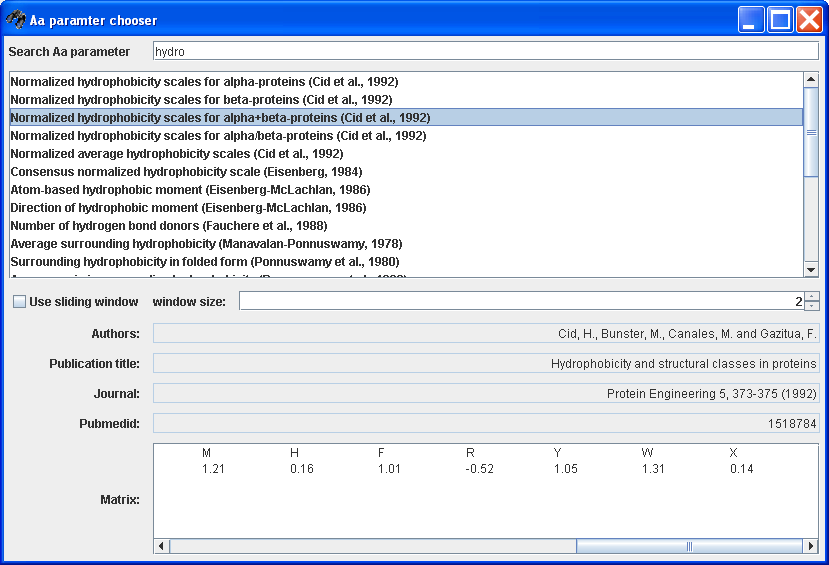
\includegraphics[scale=0.8]{Aa_paramter_chooser.png}
\caption{The amino acid parameter chooser panel.}
\label{Aa_paramter_chooser}
\end{center}
\end{figure}

\paragraph{}The size and the usage of the sliding window can be set in this panel by changing the spinner. The default size is 3.

\section{Saving the output visualization panels}
\paragraph{}The different panels created with iceLogo can be saved to a \textit{.pdf} file. A save selection panel, where specific visualization panels can be selected, is opened after that the \textit{save} button \includegraphics[height=5ex]{save.png} is clicked.
\section{Species adder} \label{species adder}
\paragraph{} When iceLogo is run in the static mode (see \ref{static}) a Swiss-Prot species composition can be choosen to create the reference set. Not all species are listed in the drop-down menu as default. A panel can be opened where other species can be added by clicking the \textit{add species} 
\includegraphics[height=5ex]{adder.png} button. This panel can be seen in figure \ref{adder}.

\begin{figure}[H]
\begin{center}
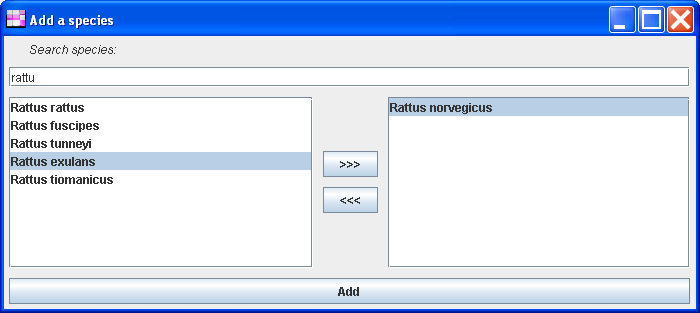
\includegraphics[scale=0.8]{adder_panel.png}
\caption{New species can be added with this panel.}
\label{adder}
\end{center}
\end{figure}

\paragraph{}In the search text field at the top of the panel a part of the scientific name of the species can be typed. The corresponding species will be listed in the left list. Species can be added to the right list by selecting these and clicking the \textit{$>>>$} button. By clicking \textit{add} at the bottom of the panel, the species in the right list will be added to the iceLogo program and can be choosen to create the reference set. After adding the new species the program should be restarted.


%chapter with the google group site
\chapter{Problems and questions}
\paragraph{}A google discussion group (\url{http://groups.google.com/group/iceLogo}) was created for problems and questions. Also, if you have a request (a new visualization style, \ldots) you can post a message on the google discussion group.


\backmatter

\end{document}